% ========== Config ========== %

\documentclass{article}

\usepackage{fancyhdr} % draw header and footer separations
\usepackage{lastpage} % get last page number
\usepackage[super]{natbib} % format references
\usepackage{url} % pretty wrap url
\usepackage{indentfirst} % indent every paragraph
\usepackage{hyperref} % color url + ref sections
\hypersetup{urlcolor=blue, colorlinks=true}
\usepackage{pythonhighlight} % python syntax highlighting
\usepackage{adjustbox} % resize overful tables
\usepackage{amsmath} % equations
\usepackage{amssymb} % symbols
\usepackage{graphicx} % images
\usepackage[left=2cm, right=2cm, bottom=3cm, top=3cm]{geometry} % margin settings
\renewcommand{\ttdefault}{txtt}


\pagestyle{fancy}
\fancyhead[L]{DAT 510 - Security and Vulnerability in Networks}
\fancyhead[R]{Assignment 3}
\fancyfoot[C]{ \thepage / \pageref{LastPage} }
\fancyfoot[L]{ T\'eo Bouvard }

\renewcommand{\headrulewidth}{0.4pt}
\renewcommand{\footrulewidth}{0.4pt}


% ========== Meta ========== %

\title{\textbf{Blockchain}}
\author{}
\date{}

% ========== Document ========== %

\begin{document}

\maketitle \thispagestyle{fancy}

\begin{abstract}
    In this assignment, we implement a basic blockchain allowing users to create transactions, add transactions to a block, and add blocks to a chain. We also implement a MD5 hashing function to generate all necessary hashes in the blockchain. In the \nameref{Research} section, we discuss a general overview of the blockchain technology, its consensus protocols and the importance of digital signature in such systems.
\end{abstract}

\section{Introduction}

Although the first research describing a chain of blocks linked together using cryptography traces back to Haber et al.\cite{Haber1991} in 1991, it was only practically implemented in 2008 by an unknown individual (or group of individuals) named Satoshi Nakamoto\cite{nakamoto2012bitcoin}. Nakamoto released the software on January 2009, effectively creating the first public cryptocurrency blockchain, the Bitcoin. The complete software is quite complex, as it comprises a consensus mechanism among a peer-to-peer network, but how can its core functionality be broken down to a simple Python implementation ?

\section{Design and Implementation}

The implementation contains two main modules : \verb+hash.py+ and \verb+blockchain.py+. The \verb+hash.py+ module contains an implementation of the MD5 function as specified in RFC 1321 \cite{RFC1321}. Its main function \verb+md5()+ is used as the hash function in the rest of the program. It takes a \verb+bytes+ object as input and outputs its 64 bits message digest in hexadecimal format. The \verb+blockchain.py+ module contains the classes used to model a blockchain : Blockchain, Block, Transaction and MerkleTree.

\bigskip

The conceptual base class is the Transaction, which comprises a timestamp, a sender, a receiver and a value. Once instantiated, Transaction objects can be added to Block objects, which contains a block number, a creation timestamp, the previous block's hash (once added to the chain) and the transaction root. The transaction root is a MerkleTree object containing all transactions and their respective hashes, as well as the root hash which is computed each time a new transaction is added to the block. The root hash follows the properties of a Merkle Tree\cite{wiki:merkletree}. Once a user is done adding Transactions to a Block he can add the block to a Blockchain object, at which point the previous block hash is written to the added block.

\bigskip

The strategy used to hash complex objects is to concatenate their relevant attributes into a single string and hash the string's utf-8 encoding representation.

\bigskip

The root of the Merkle Tree is computed recursively in its \verb+compute_root()+ class method. This method hashes a list of transactions by grouping consecutive transactions into pairs, hashing their concatenation and appending the result to a new list. The function calls itself with this new list as a parameter until the list only contains one element, which is the root hash of the Merkle Tree.

\bigskip

If the \verb+VERBOSE+ variable is set to true in the \verb+blockchain.py+ file (it is, by default), every action is logged to the standard output. A graphical representation of the chain can be displayed directly by printing the chain (also done by default). To run a demo, simply use \verb+make demo+. In the \verb+demo.py+ file, the \verb+SLEEP_TIME+ variable can be set to an integer number of seconds to run the demo at a slower pace.

\section{Test Results}

The following tests can be reproduced by running the \verb+make tests+ command.

\begin{table}[h]
    \begin{center}
        \begin{adjustbox}{width={\textwidth},totalheight={\textheight},keepaspectratio}
        \begin{tabular}{|c c c|} 
            \hline
            \textbf{Plaintext} & \textbf{Hash} & \textbf{Matches RFC test} \\
            \hline
             & 0xd41d8cd98f00b204e9800998ecf8427e & \checkmark \\
            a & 0x0cc175b9c0f1b6a831c399e269772661 & \checkmark \\
            abc & 0x900150983cd24fb0d6963f7d28e17f72 & \checkmark \\
            message digest & 0xf96b697d7cb7938d525a2f31aaf161d0 & \checkmark \\
            abcdefghijklmnopqrstuvwxyz & 0xc3fcd3d76192e4007dfb496cca67e13b & \checkmark \\
            ABCDEFGHIJKLMNOPQRSTUVWXYZabcdefghijklmnopqrstuvwxyz0123456789 & 0xd174ab98d277d9f5a5611c2c9f419d9f & \checkmark \\
            12345678901234567890123456789012345678901234567890123456789012345678901234567890 & 0x57edf4a22be3c955ac49da2e2107b67a & \checkmark \\
            \hline
        \end{tabular}
    \end{adjustbox}
    \end{center}
    \caption{Comparing MD5 test suite to our implementation} \label{tab:aes}
\end{table}

This demo can be reproduced (beware, the number of blocks and transactions are random) using the \verb+make demo+ command.

\begin{figure}[h!]
    \begin{center}
        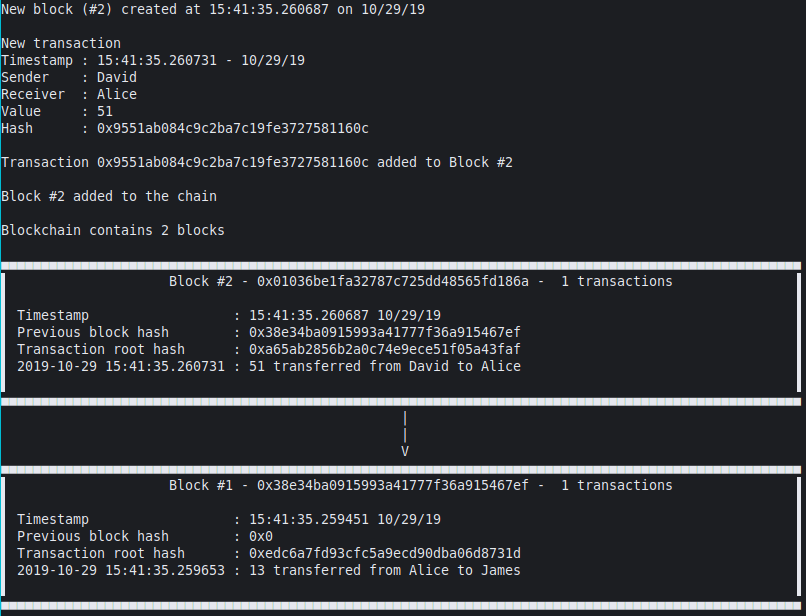
\includegraphics[width=0.7\linewidth]{img/demo.png}
        \caption{Extract of a demo run of the implementation}
        \label{fig:demo}
    \end{center}
\end{figure}


\section{Research}\label{Research}

According to Wikipedia\cite{wiki:blockchain}, a blockchain is a growing list of records, called blocks, that are linked together using cryptography. Each block contains a cryptographic hash of the previous block, a timestamp, and transaction data. The transaction data is generally represented as a Merkle tree, which allow efficient and secure verification of the contents of large data structures.

\bigskip

A blockchain can be used as a distributed ledger, as its design makes it resistant to data alteration. Each block being linked to the previous one by its cryptographic hash, modifying transaction data in one block would require a modification of every subsequent block, which requires consensus of the network majority. This design solves some of the long-standing problems of digital currencies, such as the double-spending problem, without the need of a trusted third-party authority. The decentralized design of this system makes it secure by not having a central point of failure, whereas traditional databases may be subject to exploits because all the data is held centrally.

\bigskip

Blockchains can be permissionless (open) which means anyone can add records to it, or permissioned (private), in which case the access to the chain is restricted to authorized users only. In open blockchains, access control is usually done by consensus mechanisms in order to limit the number of new blocks added to the chain. In the case of the Bitcoin blockchain, the consensus mechanism used is a Proof of Work.
Private blockchains, on the other hand, do not benefit from the network advantages, and are closer in design to traditional databases.

\bigskip

To achieve overall reliability in blockchains, such systems rely on consensus protocols. These protocols dictate the policy of acceptance of new blocks within the chain. The most commonly used consensus protocols are Proof of Work (PoW) and Proof of Stake (PoS), which are described below.

\bigskip

The main idea behind Proof of Work is that the requester of a service must prove that it has performed a measurable effort in order to submit its request. In blockchains, this effort is to solve a Hashcash-like\cite{back2002hashcash} cryptographic puzzle. By solving such a puzzle, a user can prove that it has performed a computationally expensive task, which can be easily verified by the service provider.


Let's take the Bitcoin blockchain as an example. In order to add a block to this chain, a network of users must ``mine'' it by discovering a nonce which, when hashed together with the current block, produces a hash value below a defined target value. To do so, miners have no other choice than to bruteforce different nonces until the hash value begins with the necessary amount of zeros. Once this nonce is discovered the new block can be added to the chain, and other users can verify with little effort that the cryptographic puzzle has been correctly solved. In the Bitcoin blockchain, a double SHA-256 is used as hash function, and the numbers of leading zeros of the target values depends on the current difficulty of the blockchain, which regulates the average amount of time it takes to find a new block to around 10 minutes.

\bigskip

On the other hand, Proof of Stake does not rely on computationally intensive tasks in order to add blocks to the chain, but chooses the next block based on random selection combined with different factors such as wealth or age of the candidate requests. In Peercoin's blockchain for example, the account allowed to forge the next block is chosen by a randomized combination of the amount of coins held and the amount of time these coins have been held (their age). A direct advantage of PoS over PoW is that it does not require the huge amount of processing power necessary to solve PoW cryptographic puzzles, and this processing power often comes from electricity generated from non-renewable sources of energy. However, PoS is much more complex to implement securely and reliably than PoW. It is less widely used in public blockchains, and only a few cryptocurrencies use it as their consensus protocol.

\bigskip

There exists some other consensus protocols such as Proof of Space, Proof of Authority or Proof of Burn. As of 2019, they are even less used than Proof of Stake because of some loopholes such protocols may contain.

\bigskip

In order to function properly, blockchain systems rely heavily on asymmetric cryptography. Each transaction contained in a block is signed by the private key of the sender. This allows every user of the network to verify the authenticity of a transaction, and solves the double spending problem by preventing repudiation of the transaction. Asymmetric cryptography is also used to derive the address of users, which are a hash of their public key combined with other information such as checksums of the network properties when the key pair is generated. This demonstrates the usefulness of digital signatures in the context of blockchains.


\section{Discussion}

Although MD5 was considered a secure hash function in 1992, a 2013 cryptanalytic attack by Xie Tao et al.\cite{xie2013md5} allows to find collisions in $2^{18}$ MD5 compressions, which takes around one second on an average computer. This would make our blockchain implementation vulnerable to malicious block forgery, and bruteforce would not be the most efficient PoW algorithm anymore. This is why actual public blockchains use more secure hash functions such as double SHA-256 in the case of Bitcoin.

\bigskip

Implementing a hash function is also a bad idea in general as it is prone to errors, so in a production setting using publicly available libraries would be preferable. However, having to implement MD5 from the specification is a good exercise in specification-to-code translation. Implementing a more secure hash function such as SHA-3 would have taken a lot more time, and was outside the scope of this assignment.

\bigskip

In this implementation, we use names to identify users in transactions. This is obviously not the right way to do it in a secure blockchain, because it does not provide any non-repudiation protection. One possible secure implementation would be to use asymmetric cryptography, as it is done in the Bitcoin chain, and sign every transaction with the sender's private key. This would prevent double-spending problems because users could not deny having made a transaction.

\section{Conclusion}

In this assignment we familiarized ourselves with blockchain systems, implementing a stripped-down yet functional proof-of-concept blockchain in Python. We also implemented a hash function from its specification, and identified the weaknesses it includes in our software. Finally, we got an overview of the different kinds of blockchains, their consensus mechanisms and the importance of digital signatures in this field.


\bigskip

% ========== References ========== %

\bibliographystyle{unsrtnat}
\bibliography{sources}

\end{document}



